\graphicspath{{evil-ndi/}}

\chapter{Learning \texorpdfstring{``Evil''}{"Evil"} Non-Representative Climate Numbers}
\label{chap:evilndi}

As described above, there is some debate surrounding the value of scientific or
numeric information regarding climate change. Indeed, some have claimed that
such interventions will only serve to polarize individuals, thus making the
situation worse than it already is. However, some organizations publish
out-of-context facts to try to undercut the reality or gravity of human-caused
climate change. Such numbers are often blatantly cherry picked. For example, the
Earth’s temperature decreased (by 0.2oF) from 1940 to 1975 (Jastrow, Nierenberg,
\& Seitz, 1991). This surprising fact, though, hardly contradicts the ever more
obvious warming trend over the last 125+ years, as one can pluck many ``trends''
in noisy time series by picking endpoints that are oddly high or low. Given this
rather clear intent to mislead (Oreskes \& Conway, 2010), we (partly
tongue-in-cheek) label these numbers ``evil.'' 

Our three hypotheses were that misleading facts would reduce:
\begin{enumerate}
    \item participants’ climate change acceptance, 
    \item ratings of their knowledge of the issue, and 
    \item their climate-change funding preferences.
\end{enumerate}
Of course, lest we erode participants’ acceptance of anthropogenic climate
change more than fleetingly, we debriefed them right afterward with more
complete information---including the mechanism and a large dose of relevant
facts. It should be clear that we're not interested in perfecting this approach! 

Here we go into the much more easily obtained effects we demonstrated using the
anti-climate NDI. This is much shorter, as we were mostly curious to see if we
could get an effect. In particular, we only did one experiment with one
undergraduate seminar course (where we could be sure to administer a proper
debriefing).

\section{Study: UC classroom intervention with \texorpdfstring{“evil”}{"evil"}
    numbers}

\subsection{Methods} 
\label{sec:evilndi-methods}

\subsubsection{Materials and Procedure}

Participants were engaged in one of two similar misleading numeracy
interventions. In both versions, survey methods were as described in
Chapter~\ref{chap:survey}. This study utilized a somewhat compact version of a
pre- and post-intervention test using only the 14 items in
Table~\ref{table:rtmd-questions} (up through \textsf{engage}), plus a
self-rating of climate-change knowledge.  

In the “no pre-test blast” version of the intervention, participants estimated
each of eight items prior to receiving the feedback values, with an emphasis on
maximizing the quantity of feedback numbers presented to the participant. To
this end, this eight-item survey included only a post-test (i.e., no pre-test),
and lacked a policy component (thus, it was an EI intervention, lacking ``P'' or
``C'', simlar to the approach used in Chapter~\ref{chap:two}). 

A more comprehensive engagement containing only two items was administered to
the rest of the class. This version included a pre-test and additional questions
about each item. In addition, we asked students about their surprise level after
each feedback value and requested both their climate-change funding Policies and
post-feedback policy Changes versus various UNDP millennium goals.  Thus, this
latter variant was a full EPIC intervention. The same set of alternatives was
used across the 4 variants of the 2-item intervention, and these are listed
along with policy-relevant instructions in Appendix~\ref{app:undp}.

Note that while this experiment is presented first as a motivation for the
following chapters, it was actually carried out \emph{after} a number of
experiments in Chapters~\ref{chap:prondi} and \ref{chap:mechanism}. Thus, a
number of experimental design choices made here are motivated by findings from
experiments in those chapters.

\subsubsection{Participants}

Two classes of UC Berkeley undergraduates were engaged in this intervention
($N=104$). 59 students completed the 8-item “no pre-test” version of the
experiment and 45 completed the 2-item full EPIC intervention. All participants
were retained after examining the coherence of survey responses.

In the 8-item intervention, 34 participants were female and mean conservativism
of 3.64 ($sd=1.59$). In the 2-item intervention, 31 participants were female and
mean conservativism was 3.68 ($sd=1.43$). Breakdown of political party is given
in Table~\ref{table:evil-party}.

% TODO: party table 
% latex table generated in R 2.15.1 by xtable 1.7-1 package
% Tue Jun 18 14:46:50 2013
\begin{table}[ht]
\caption{Stated party affiliations for participants in “evil” NDI study (UC
    Berkeley undergraduates).}
\label{table:evil-party}
\centering
\begin{tabular}{rrr}
  \toprule
     & 8-item & 2-item \\ 
  \midrule
  democrat &  20 &  21 \\ 
  republican &   4 &   2 \\ 
  green &   1 &   0 \\ 
  libertarian &   1 &   3 \\ 
  independent &   6 &   2 \\ 
  none &  21 &  13 \\ 
  other &   1 &   1 \\ 
  decline to state &   5 &   3 \\ 
   \bottomrule
\end{tabular}
\end{table}
\subsection{Results}

% TODO: Also note changes for each item / individual comparisons here (if you
% have time / people want)
Overall, these numbers had a profound impact, the details of which are described
below. As with other NDI interventions, and consistent with our pilot testing,
individuals generally found each of these items surprising, ranging from
surprise ratings of 5.83 to 8.53 across both interventions. Mean surprise
ratings were 6.03 for the 2-item intervention and 6.62 for the 8-item
intervention. Ratings were on a 1--9 scale, with all ratings above “1”
indicating some level of surprise.

\subsubsection{Shifts away from GW policy preferences}

As hypothesized, policy preferences for funding UN goals related to climate
change dropped ($\chi^2(1)=22$, $p<0.01$) for all eight funding priorities.
(Unfortunately for global warming as a social priority, the highest mean
pre-test preference for funding climate change initiatives reached only a 50-50
split of available funds.) These results are depicted in
Figure~\ref{fig:evil-alloc}. While, due to time constraints, we did not check
for a similar result in our 8-item intervention, it seems likely that similar
(or greater) shifts would occur along with the much more drastic GW attitude
shifts we'll see below.

\begin{figure}
    \centering
    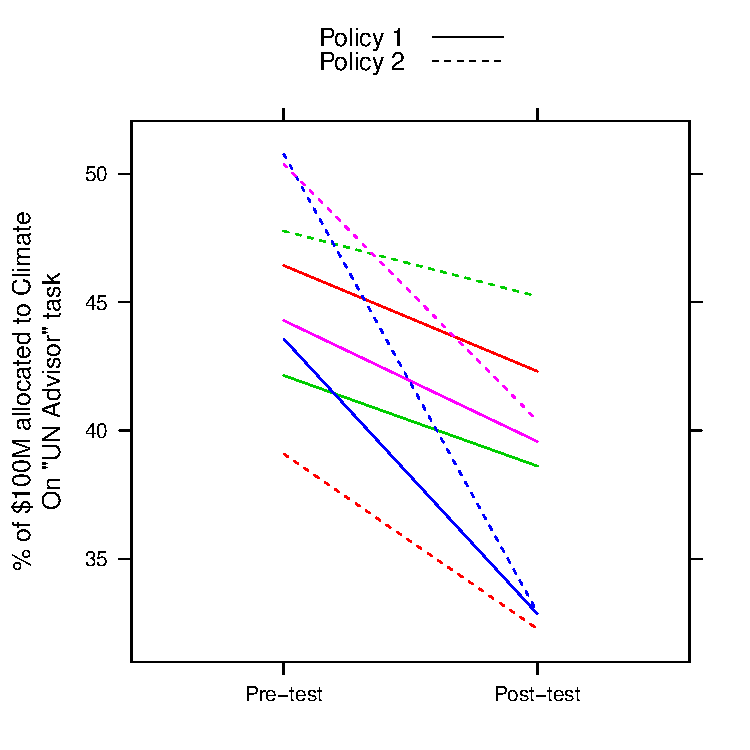
\includegraphics{evil-alloc.pdf}
    \caption{Preference for allocation of \$100M on “UN Advisor” task. Values
        are expressed as a percentage of funds that were allocated to
        climate-relevant projects vs. projects supporting an alternative UNDP
        millenium goal.}
    \label{fig:evil-alloc}
\end{figure}

\subsubsection{GW acceptance eroded by misleading numbers}

Also, as hypothesized, mean climate change acceptance dropped significantly,
from 6.5 on the pre-test to 6.2 on the post-test for the two-item group (6\% of
available room, for a 9-point scale, $t(42)=-4.3$, $p<0.001$), and significantly to
5.9 for the eight-item group (12\% of available room, $t(88.6)=‑2.61$, $p<0.005$).
Note that these shifts were also in the direction of ambivalence (a ``5''
rating), and may reflect confusion rather than disagreement. Mean ratings are
depicted in Figure~\ref{fig:evil-GW}.

\begin{figure}
    \centering
    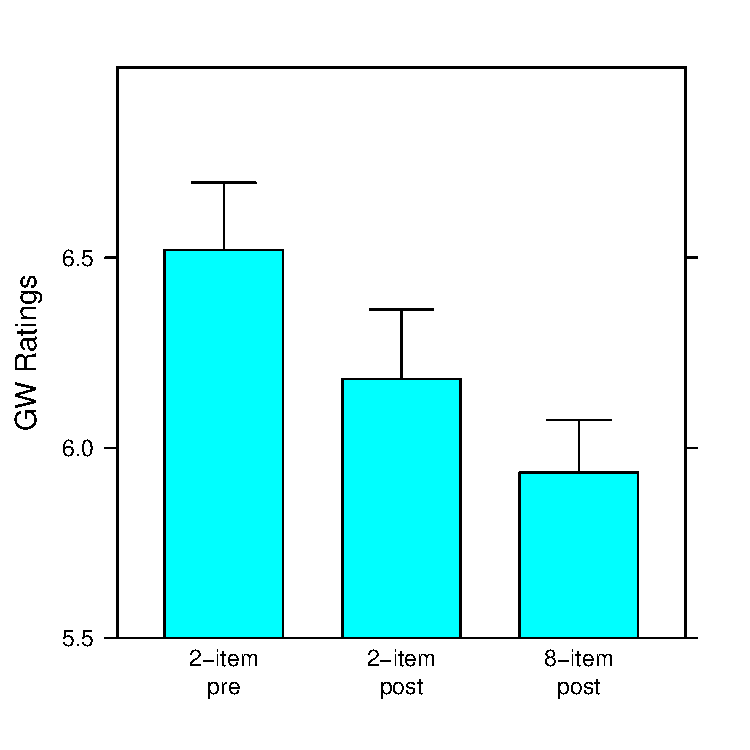
\includegraphics{evil-GW.pdf}
    \caption{Mean ratings for GW survey items on pre- and post-test. Pre-test
        surveys were only administered for the 2-item group, but should be
        indicative of population responses.}
    \label{fig:evil-GW}
\end{figure}

\subsubsection{Self-confidence in GW knowledge eroded by misleading numbers}

Our third hypothesis was also supported, as self-rated knowledge dropped from a
mean of 5.0 on the pre-test to 4.5 for the two-item group (12\% of available
room, $t(44)=-2.5$, $p<0.01$), and plummeted to 2.9 on eight-item survey
($t(87.2)=-5.3$, $p<0.001$). This latter decrease, 2.1, represents 53\% of the
available room to drop on a 9-point scale, which is exceptionally large. These
ratings are depicted in Figure~\ref{fig:evil-know}.

\begin{figure}
    \centering
    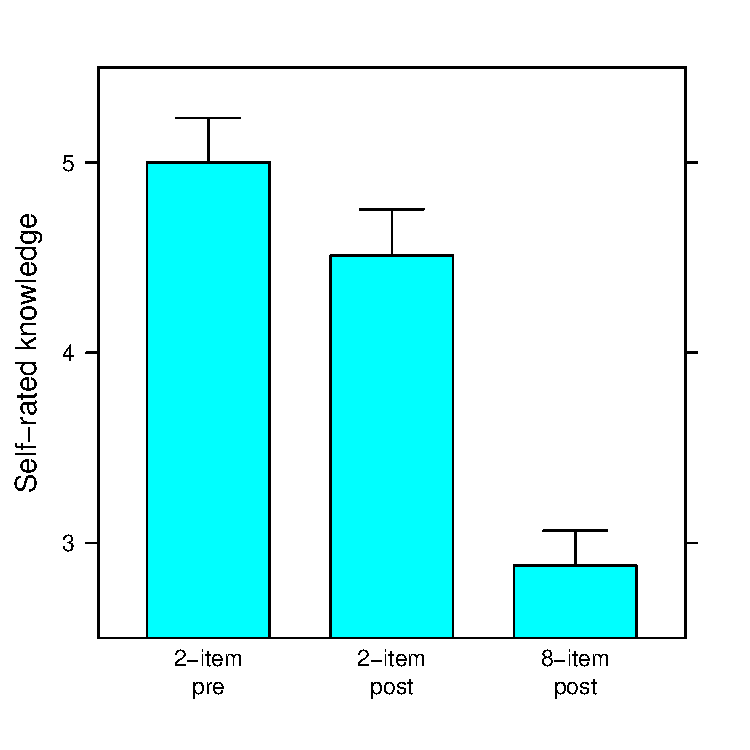
\includegraphics{evil-know.pdf}
    \caption{Self-rated knoweldge for individuals on pre- and post-tests. Again,
        pre-tests were only administered to individuals in the 2-item
        experimental variant.}
    \label{fig:evil-know}
\end{figure}

\subsection{Discussion}

In stark contrast to arguments that numeracy is polarizing \parencite{kahan}, we
have provided an existence proof that appropriately selected scientific facts
can have a profound effect in eroding the existing beliefs of a population
(i.e., “liberals” can be pushed in a more “conservative” direction). In
particular, we have demonstrated marked erosion of self-confidence in one's own
knowledge, as well as belief and concern regarding anthropogenic climate
change---even in our relatively liberal and
anthropogenic-climate-change-acceting sample of UC Berkeley undergraduates.
Such results were observed with as little as \emph{two} numbers.
% Still need to grab stuff from above
Consider the effect of the writings of \textcite{mueller}, a prominent professor
at our ostensibly liberal institution. We must assume that educated, liberal
individuals may be easily swayed by a small dose of factual (but
non-representative) numerical or scientific information from such a source.

A central point illustrated by this study is that individual's understandings
are demonstrably fragile. Even an intervention of a few minutes can massively
undercut individual's confidence in thier own knowledge, along with overall
belief and concern about global climate change.

% TODO: There are two points here, one about the difference between self-guided
% and directed education, and one about the ability of scientific information to
% work for both sides of the climate “debate”
A secondary point to consider is that, As noted by \textcite{kahan,mccright},
individuals tend to be little-affected by self-guided educational efforts. Thus,
one might conclude that climate change accepters are unlikely to come into
contact with such numbers on their own.  However, there are concerted efforts to
distribute such numbers on the internet and elsewhere. As shown above and as
noted by \cite{mccright}, scientific information might push individuals both
towards scientific consensus, as well as \emph{away} from it.  Thus, it seems
wise to build a solid foundation of climate change-relevant knowledge in the
American populace. 

It is clear that even relatively educated members of the public (e.g.,
undergraduates at a top-tier university) are highly susceptible to misleading,
cherry picked facts. Such facts are clearly known to organizations attempting to
undermine the overwhelming scientific consensus about climate change. Thus,
cognitive science must counter the increasing sophistication with which such
organizations distribute misleading information.

\section*{Acknowledgements}

The work reported in this chapter has been previously published, in part, in
\textcite{clark_knowledge_inpress}.  All such material is re-used here with the
permission of my co-authors, the publishers, and the Graduate Division at the
University of California, Berkeley.
